% Compile with latex, then dvisvgm --no-fonts --exact --bbox=papersize.
\documentclass[tikz,border=8pt]{standalone}
\usepackage[T1]{fontenc}
\usepackage{lmodern}
\begin{document}
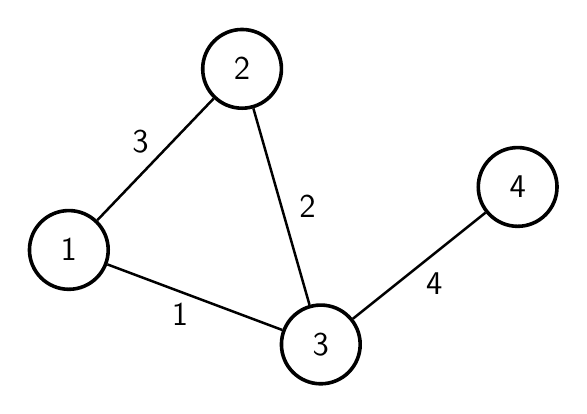
\begin{tikzpicture}[
    font=\sffamily\large,
    vertex/.style={circle,draw,line width=1.3pt,fill=white,
                   minimum size=10mm,inner sep=0pt},
    edge/.style={line width=0.9pt},
    weight/.style={inner sep=2pt}]
  \node[vertex] (1) at (0,0) {1};
  \node[vertex] (2) at (2.2,2.3) {2};
  \node[vertex] (3) at (3.2,-1.2) {3};
  \node[vertex] (4) at (5.7,0.8) {4};
  % The edge of weight 3 is absent from every minimum spanning tree.
  \draw[edge] (1) -- node[weight,above left] {3} (2);
  \draw[edge] (1) -- node[weight,below left] {1} (3);
  \draw[edge] (2) -- node[weight,right=4pt] {2} (3);
  \draw[edge] (3) -- node[weight,below right] {4} (4);
\end{tikzpicture}
\end{document}
